\documentclass[aspectratio=169,11pt]{beamer}
\usepackage{beamertemplate}
% --- estilo de comandos (consistente con el resto del temario) ---
\newcommand{\cmd}[1]{\texttt{\color{uznavy}#1}}
\newcommand{\cmdbox}[1]{%
  \begin{center}%
  {\setlength{\fboxsep}{6pt}\colorbox{uzlav!40}{\parbox{0.88\linewidth}{\ttfamily\footnotesize #1}}}%
  \end{center}}
% --- rótulo de subtema dentro de una sección ---
\newcommand{\subt}[1]{{\color{uznavy}\bfseries #1}\par\smallskip}
\usepackage{graphicx}
\usepackage{url}
\usepackage{textcomp}
\usepackage{eurosym}
\usepackage{booktabs}
\usepackage[normalem]{ulem}
\usepackage{ragged2e}
\usepackage{etoolbox}
\apptocmd{\itemize}{\justifying}{}{}
\AtBeginEnvironment{frame}{\justifying}

% Repite el índice al empezar cada sección, resaltando la que comienza
\setbeamertemplate{section in toc shaded}[default][30]
\AtBeginSection[]{%
  \begin{frame}{Índice}
  \footnotesize
  \tableofcontents[currentsection]
  \end{frame}
}

\title[SSI -- Tema 3.4]{Denegación de Servicio (DoS)}
\subtitle{Seguridad en Sistemas Informáticos --- Tema 3.4}
\author{José Luis Martínez}
\institute{Universidad de Castilla-La Mancha}
\date{Curso 2026/27}

% --- build reproducible / metadatos limpios ---
\pdfinfoomitdate=1
\pdftrailerid{}
\pdfsuppressptexinfo=-1

\begin{document}

\begin{frame}[plain]\titlepage\end{frame}


\section{Introducción}

\begin{frame}{Introducción}
\vspace{-0.5em}
\begin{center}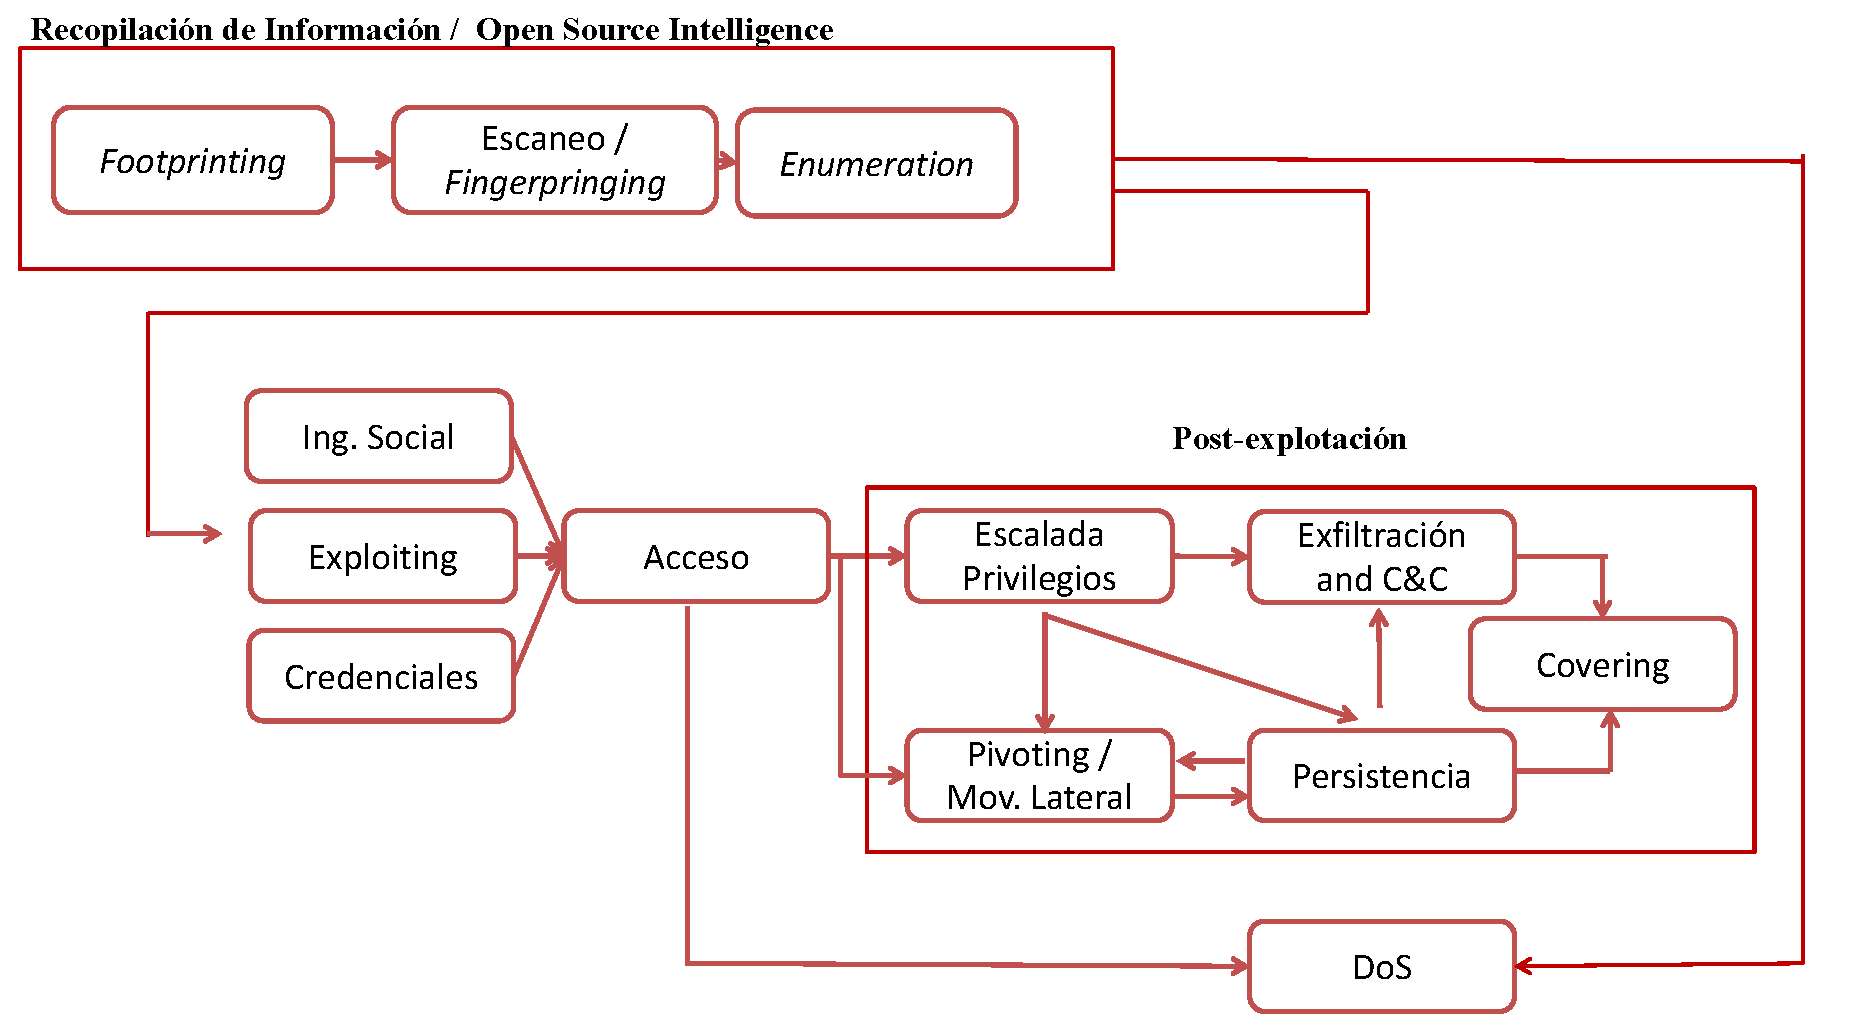
\includegraphics[width=\textwidth,height=0.80\textheight,keepaspectratio]{img/taxonomia-ataque.pdf}
\end{center}
\end{frame}

\begin{frame}[allowframebreaks]{Introducción}
\small
\subt{Los dos grandes vectores de ataque}
  \begin{itemize}
  \item Tras la fase de recopilación de información, en la que se han identificado los activos de la organización, los dos principales vectores de ataque son:
  \item \textbf{Ataques de acceso} (objetivo principal de un pentesting)
    \begin{itemize}
    \item Se han visto en profundidad en los temas anteriores: credenciales, ingeniería social y explotación de vulnerabilidades
    \end{itemize}
  \item \textbf{Denegación de servicio (DoS)}
    \begin{itemize}
    \item A diferencia de los ataques de acceso, que pretenden entrar en un sistema, aquí el objetivo es dejarlo inutilizado para que nadie pueda usarlo
    \item No compromete la confidencialidad ni la integridad: ataca directamente a la \textbf{disponibilidad}, el tercer pilar de la tríada CIA
    \end{itemize}
  \end{itemize}
\end{frame}

\begin{frame}[allowframebreaks]{Introducción}
\small
\subt{Qué es un ataque DoS}
  \begin{itemize}
  \item Los ataques DoS buscan que un recurso de red (un host, un servicio o la propia red de interconexión) reduzca su rendimiento, restrinja el servicio o deje de funcionar para los usuarios legítimos
  \item Una de las formas más comunes de perpetrarlo es la inundación (\emph{flooding}) de peticiones, hasta saturar la capacidad de respuesta del recurso
  \end{itemize}
\vspace{-0.5em}
\begin{center}
\includegraphics[width=0.72\textwidth,height=0.47\textheight,keepaspectratio]{img/sl005_1.png}
\end{center}
\end{frame}

\begin{frame}[allowframebreaks]{Introducción}
\small
\subt{De DoS a DDoS}
  \begin{itemize}
  \item Los ataques DoS distribuidos (DDoS) persiguen el mismo objetivo que los DoS, pero su impacto y su probabilidad de éxito son mucho mayores: parten de una multitud de sistemas comprometidos (\emph{zombies}), normalmente organizados en una \emph{botnet}. Estos bots son gobernados por el atacante mediante un sistema de mando y control (C\&C)
  \end{itemize}
\vspace{-0.5em}
\begin{center}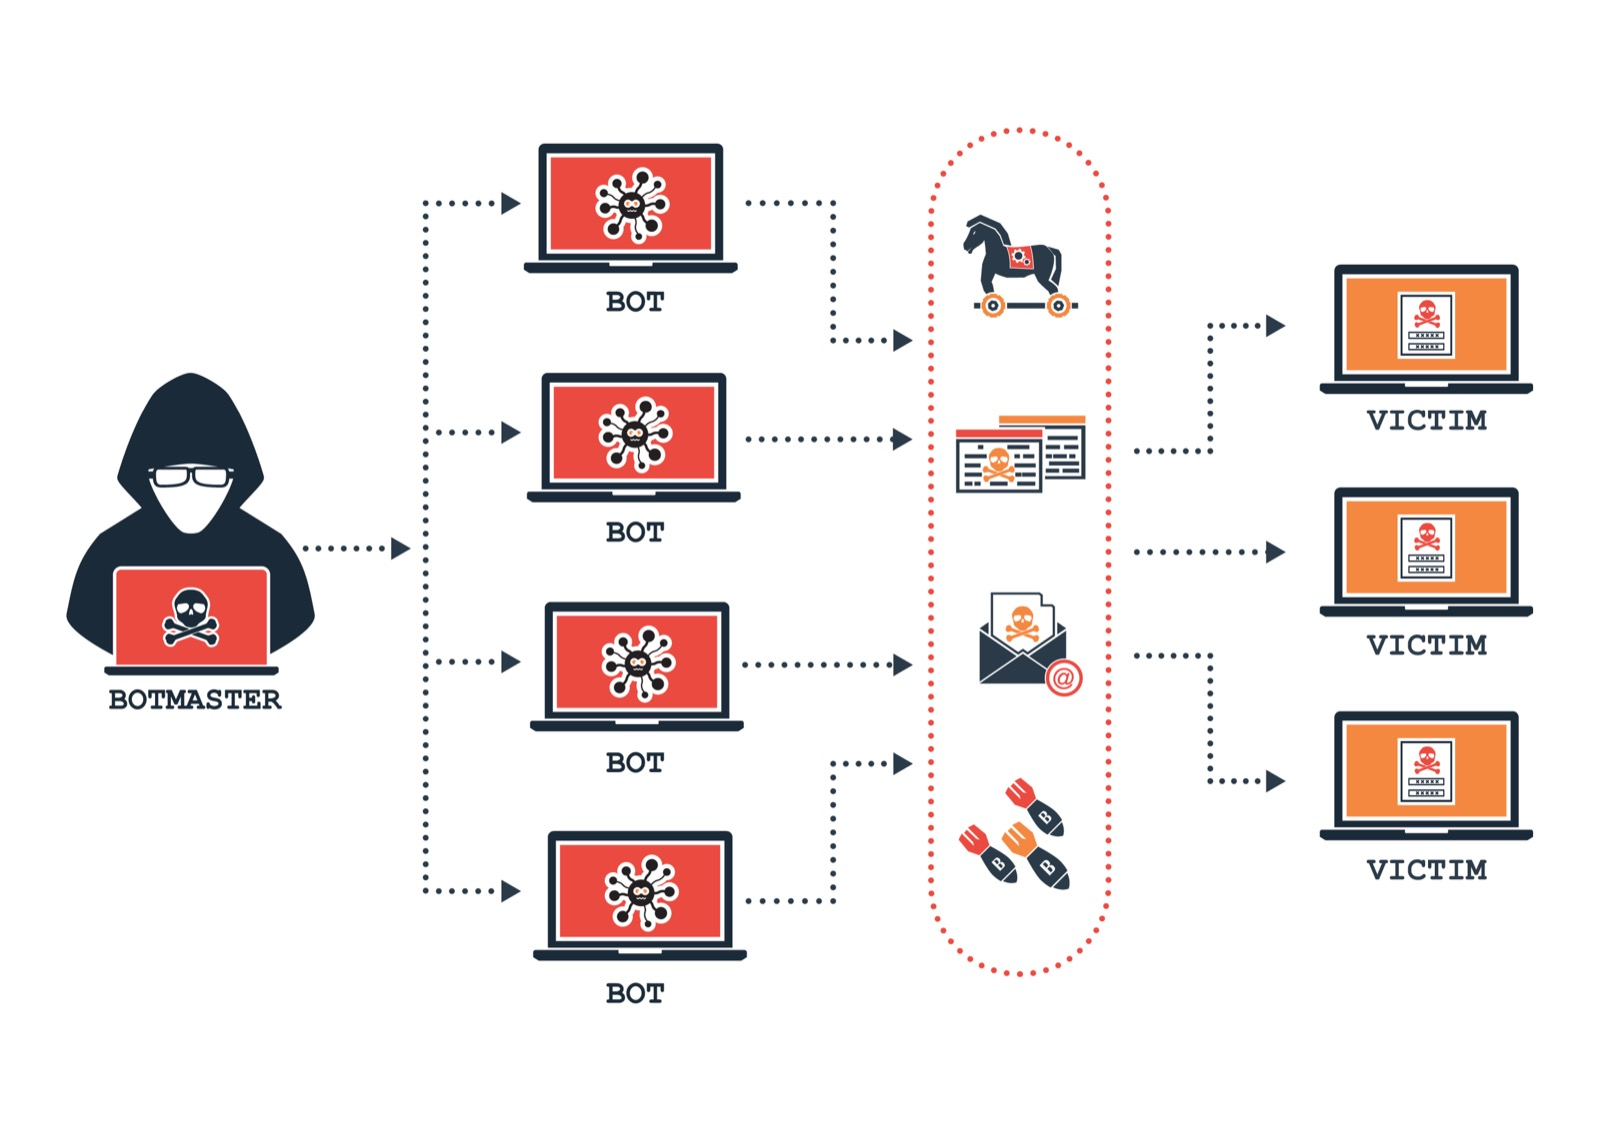
\includegraphics[width=0.74\textwidth,height=0.52\textheight,keepaspectratio]{img/ddos_incibe.jpg}
\end{center}
\end{frame}

\begin{frame}[allowframebreaks]{Introducción}
\small
\subt{El objetivo final de un ataque DoS}
  \begin{itemize}
  \item Consumo de recursos: ancho de banda, memoria, disco, CPU o descriptores de fichero
  \item Agotamiento de tablas de estado en cortafuegos, balanceadores y sistemas operativos
  \item Ataques físicos de destrucción o alteración de componentes
  \item Destrucción de ficheros de configuración o de programas del host
  \item Daño reputacional y económico: el coste de la indisponibilidad suele superar al del incidente técnico
  \end{itemize}
\end{frame}

\begin{frame}[allowframebreaks]{Introducción}
\footnotesize
\subt{Caso de estudio: caída de WhatsApp, Facebook e Instagram (4 de octubre de 2021)}
  \begin{itemize}
  \item No fue un ataque DoS, sino una \textbf{autodenegación de servicio}: el efecto sobre los usuarios fue idéntico al de un DDoS masivo (unas 6~h de caída global).
  \item Cloudflare observó a las 15:40~UTC un pico de cambios de rutas BGP en los sistemas autónomos de Facebook y, a las 15:58~UTC, que Facebook había dejado de anunciar las rutas hacia sus prefijos de DNS: sin ellas, ningún resolutor del mundo podía llegar a sus servidores de nombres.
  \item Meta confirmó después la causa: durante un mantenimiento rutinario se ejecutó un comando que debía evaluar la capacidad del \emph{backbone} y que tumbó todas las conexiones entre sus centros de datos; un fallo en la herramienta interna de auditoría no impidió que se ejecutase. Al quedar aislados los DNS, éstos retiraron sus anuncios BGP.
  \item \textbf{Lección}: la disponibilidad depende tanto del atacante como de la propia gestión del cambio.
  \item Referencias:
    \begin{itemize}
    \item \href{https://blog.cloudflare.com/october-2021-facebook-outage/}{Cloudflare --- \emph{Understanding how Facebook disappeared from the Internet}}
    \item \href{https://engineering.fb.com/2021/10/04/networking-traffic/outage/}{Meta --- \emph{Update about the October 4th outage}} y \href{https://engineering.fb.com/2021/10/05/networking-traffic/outage-details/}{\emph{More details about the October 4 outage}}
    \end{itemize}
  \end{itemize}
\end{frame}

\begin{frame}[allowframebreaks]{Introducción}
\small
\subt{Tipos de ataques de DoS que veremos en el tema}
  \begin{itemize}
  \item \textbf{Volumétricos} --- agotan el ancho de banda (inundación UDP/ICMP, Smurf, amplificación)
  \item \textbf{De consumo} --- agotan recursos del host (SYN flood, fragmentación, capa~7)
  \item \textbf{Buffer overflow} --- provocan el fallo de la aplicación o del sistema
  \item \textbf{Permanentes o phlashing} --- dañan el hardware de forma irreversible
  \end{itemize}
\vspace{-0.5em}
\begin{center}
\includegraphics[width=0.70\textwidth,height=0.47\textheight,keepaspectratio]{img/sl008_1.jpg}
\end{center}
\end{frame}

\begin{frame}{Introducción}
\small
\subt{Aviso legal y ético}
  \begin{itemize}
  \item Lanzar un DoS contra un sistema ajeno \textbf{sin autorización expresa y por escrito} es delito en España: el art.~264~bis del Código Penal castiga con prisión de seis meses a tres años a quien obstaculice o interrumpa gravemente el funcionamiento de un sistema informático ajeno.
  \item Los ejercicios de este tema se realizan \textbf{exclusivamente} sobre las máquinas del laboratorio (Metasploitable2, Windows~XP/7 en red aislada).
  \item Nunca se lanzan pruebas contra servicios en producción, redes del campus ni servicios de terceros, aunque sean propios: un DoS puede afectar a toda la infraestructura compartida.
  \item Referencia: \href{https://www.boe.es/buscar/act.php?id=BOE-A-1995-25444}{Código Penal (texto consolidado, BOE-A-1995-25444)}
  \end{itemize}
\end{frame}


\section{Ataques volumétricos}

\begin{frame}[allowframebreaks]{Ataques volumétricos}
\small
\subt{Concepto}
  \begin{itemize}
  \item El objetivo de estos ataques es abusar del ancho de banda disponible entre el objetivo (normalmente el servidor) y sus usuarios legítimos.
  \item Se apoyan en protocolos no orientados a conexión y consisten en inundar la red con ese tipo de paquetes, hasta que el objetivo no es capaz de responder ni a los paquetes del ataque ni a los legítimos.
  \item Se pueden lanzar también de manera distribuida (DDoS), que es lo habitual hoy en día.
  \item Se miden en \textbf{bits por segundo} (bps): el récord conocido supera los 20~Tbps.
  \item Tipos que veremos:
    \begin{itemize}
    \item Inundación UDP
    \item Inundación ICMP
    \item Smurf
    \item Ataques de amplificación y reflexión
    \end{itemize}
  \end{itemize}
\end{frame}

\begin{frame}[allowframebreaks]{Ataques volumétricos}
\small
\subt{Inundación UDP}
  \begin{itemize}
  \item El objetivo es enviar un alto ratio de paquetes UDP a varios servidores con la dirección IP de origen falseada (\emph{spoofed}) con la dirección de la víctima.
  \item Estos servidores actúan como amplificadores, puesto que reenviarán las respuestas a la IP de la víctima, consiguiendo que ésta se sature y deje de funcionar.
  \end{itemize}
\vspace{-0.5em}
\begin{center}
\includegraphics[width=0.70\textwidth,height=0.50\textheight,keepaspectratio]{img/sl011_1.png}
\end{center}
\end{frame}

\begin{frame}[allowframebreaks]{Ataques volumétricos}
\small
\subt{Inundación ICMP}
  \begin{itemize}
  \item El objetivo es enviar un alto ratio de paquetes ICMP \emph{echo request} (ping) a la dirección de la víctima, de forma que consuma su ancho de banda respondiendo.
  \item También se puede hacer rebotado y amplificado (Smurf).
  \end{itemize}
\vspace{-0.5em}
\begin{center}
\includegraphics[width=0.74\textwidth,height=0.55\textheight,keepaspectratio]{img/sl012_1.png}
\end{center}
\end{frame}

\begin{frame}[allowframebreaks]{Ataques volumétricos}
\small
\subt{Smurf}
  \begin{itemize}
  \item Es similar al anterior, pero en este caso el atacante falsifica la dirección de origen del paquete ICMP con la IP del objetivo o víctima.
  \item De esta manera, todas las respuestas le llegan a la víctima y no al atacante.
  \item Se amplifica enviándolo a la dirección de \emph{broadcast} de la red: todos los equipos del segmento responden a la vez contra la víctima.
  \end{itemize}
\vspace{-0.5em}
\begin{center}
\includegraphics[width=0.64\textwidth,height=0.44\textheight,keepaspectratio]{img/sl013_1.png}
\end{center}
\end{frame}

\begin{frame}{Ataques volumétricos}
\small
\subt{Amplificación y reflexión: factores conocidos}
  \begin{itemize}
  \item Combinan \emph{IP spoofing} con servicios UDP que devuelven respuestas mucho mayores que la petición original.
  \end{itemize}
\vspace{0.3em}
\begin{center}
\footnotesize
\begin{tabular}{@{}llr@{}}
\toprule
\textbf{Servicio} & \textbf{Puerto} & \textbf{Factor de amplificación} \\
\midrule
DNS (petición \cmd{ANY} a resolutor abierto) & 53/UDP    & 28--54$\times$ \\
NTP (comando \cmd{monlist}, CVE-2013-5211)   & 123/UDP   & 556$\times$ \\
SNMPv2 (\cmd{GetBulk} a community \cmd{public}) & 161/UDP & 650$\times$ \\
SSDP (UPnP en dispositivos domésticos)       & 1900/UDP  & 30$\times$ \\
CharGEN (servicio \emph{legacy})             & 19/UDP    & 358$\times$ \\
Memcached (mayor amplificación conocida)     & 11211/UDP & 51.000$\times$ \\
\bottomrule
\end{tabular}
\end{center}
\vspace{0.3em}
{\footnotesize Fuentes: \href{https://us-cert.cisa.gov/ncas/alerts/TA14-017A}{CISA TA14-017A} y \href{https://blog.cloudflare.com/memcrashed-major-amplification-attacks-from-port-11211/}{Cloudflare --- Memcrashed}.}
\end{frame}

\begin{frame}[allowframebreaks]{Ataques volumétricos}
\small
\subt{Cómo funciona la amplificación (DNS como ejemplo)}
  \begin{enumerate}
  \item El atacante falsifica la IP de origen y pone la IP de la víctima.
  \item Envía una petición DNS de tipo \cmd{ANY} a un resolutor abierto (petición de pocos bytes).
  \item El resolutor responde con paquetes muy grandes dirigidos a la IP de la víctima.
  \item Con poco ancho de banda del atacante se genera tráfico masivo sobre la víctima, y además el origen real queda oculto (\emph{reflexión}).
  \end{enumerate}
\medskip
\subt{Detección y mitigación}
  \begin{itemize}
  \item BCP38 / uRPF: filtrado de \emph{IP spoofing} en origen, responsabilidad de los operadores (\href{https://datatracker.ietf.org/doc/html/rfc2827}{RFC 2827}).
  \item Cerrar los resolutores DNS abiertos y deshabilitar \cmd{monlist} en NTP.
  \item \emph{Rate limiting} de respuestas DNS (RRL) en el resolutor.
  \end{itemize}
\end{frame}


\section{Ataques de consumo}

\begin{frame}[allowframebreaks]{Ataques de consumo}
\small
\subt{Concepto}
  \begin{itemize}
  \item Estos ataques DoS o DDoS se basan en el consumo desmesurado de los recursos de la máquina (memoria, CPU, tablas de conexiones, etc.), derivados del uso de las conexiones del protocolo TCP o de la propia lógica de la aplicación.
  \item A diferencia de los volumétricos, no necesitan mucho ancho de banda: bastan pocos paquetes bien elegidos.
  \item Tipos que veremos:
    \begin{itemize}
    \item Inundación SYN
    \item Fragmentación
    \item Ataques de capa de aplicación (capa 7)
    \end{itemize}
  \end{itemize}
\end{frame}

\begin{frame}[allowframebreaks]{Ataques de consumo}
\footnotesize
\subt{Inundación SYN}
  \begin{itemize}
  \item El atacante envía una gran cantidad de solicitudes SYN al servidor objetivo con direcciones IP de origen falsas, creando conexiones TCP incompletas que consumen los recursos de red de la máquina.
  \item Se abusa del \emph{three-way handshake} de TCP: el atacante envía un SYN falso; el servidor responde con SYN/ACK y reserva recursos; el cliente nunca envía el ACK final y deja al servidor esperando.
  \item El host víctima lleva un seguimiento de las conexiones parcialmente abiertas en una cola de escucha, mientras aguarda los ACK que nunca llegan.
  \item Cuando la cola se llena, el sistema no puede aceptar nuevas conexiones hasta que expiran las anteriores por \emph{timeout}.
  \item Mitigación de referencia: \href{https://datatracker.ietf.org/doc/html/rfc4987}{RFC 4987 --- \emph{TCP SYN Flooding Attacks and Common Mitigations}}.
  \end{itemize}
\vspace{-0.5em}
\begin{center}
\includegraphics[width=0.56\textwidth,height=0.29\textheight,keepaspectratio]{img/sl018_1.jpg}
\end{center}
\end{frame}

\begin{frame}[allowframebreaks]{Ataques de consumo}
\small
\subt{Fragmentación}
  \begin{itemize}
  \item El atacante intenta agotar la memoria de la víctima fragmentando un paquete muy grande en muchos más pequeños, de forma que el sistema deba mantenerlos en memoria mientras intenta reensamblar el paquete original.
  \item Si los fragmentos nunca se completan, los búferes de reensamblado se llenan y el impacto es mucho mayor al incrementar la tasa de envío.
  \end{itemize}
\vspace{-0.5em}
\begin{center}
\includegraphics[width=0.84\textwidth,height=0.58\textheight,keepaspectratio]{img/sl019_1.jpg}
\end{center}
\end{frame}

\begin{frame}[allowframebreaks]{Ataques de consumo}
\small
\subt{Ataques de capa de aplicación}
  \begin{itemize}
  \item Se usan protocolos de capa de aplicación, típicamente HTTP.
  \item El atacante envía un alto ratio de peticiones \cmd{GET} o \cmd{POST} contra la víctima para saturar sus recursos y que no atienda peticiones legítimas.
  \item Se miden en \textbf{peticiones por segundo} (rps), no en bps.
  \item Un ejemplo es \emph{slowloris}: el atacante abre muchas conexiones HTTP sin completarlas, hasta alcanzar el máximo de conexiones concurrentes que soporta la víctima.
  \end{itemize}
\vspace{-0.5em}
\begin{center}
\includegraphics[width=0.62\textwidth,height=0.36\textheight,keepaspectratio]{img/sl020_1.png}
\end{center}
\end{frame}

\begin{frame}[allowframebreaks]{Ataques de consumo}
\small
\subt{Slowloris y variantes de ataques lentos}
  \begin{itemize}
  \item \textbf{Slowloris} --- abre conexiones HTTP y envía cabeceras incompletas muy lentamente, manteniéndolas vivas.
  \item \textbf{Slow POST / RUDY} --- anuncia un \cmd{Content-Length} enorme y envía el cuerpo del \cmd{POST} en bytes sueltos cada pocos segundos.
  \item \textbf{Slow Read} --- anuncia una ventana TCP de recepción cercana a cero, de modo que el servidor queda bloqueado intentando entregar la respuesta.
  \item Todos comparten la misma idea: mucho tiempo de conexión con muy poco ancho de banda, lo que los hace difíciles de distinguir de clientes lentos legítimos.
  \item Herramienta que cubre los tres vectores: \href{https://github.com/shekyan/slowhttptest}{\cmd{slowhttptest}}
  \end{itemize}
\vspace{-0.3em}
\cmdbox{slowhttptest -c 1000 -H -i 10 -r 200 -t GET -u http://\textless{}victima\textgreater{}/ -x 24 -p 3}
\end{frame}

\begin{frame}[allowframebreaks]{Ataques de consumo}
\footnotesize
\subt{HTTP/2 Rapid Reset --- CVE-2023-44487}
  \begin{itemize}
  \item Descubierto en agosto de 2023 y publicado en octubre; en su momento, el mayor ataque DDoS de capa 7 de la historia.
  \item Explota el multiplexado de HTTP/2: el atacante abre un \emph{stream} y lo cancela inmediatamente con \cmd{RST\_STREAM}, sin esperar respuesta, a velocidad extrema.
  \item El servidor ya ha asignado recursos al \emph{stream} cuando procesa el \emph{reset}, así que el coste es asimétrico: mínimo para el atacante, alto para la víctima.
  \item Cifras notificadas: Google mitigó un pico de \textbf{398 millones de peticiones por segundo}; Cloudflare, 201~millones; AWS, 155~millones. Se logró con una botnet de apenas unos 20.000 nodos.
  \item Mitigación: parches en los servidores HTTP/2 (nginx, Apache, IIS, Go \cmd{net/http}) y límites al ratio de \emph{streams} cancelados por conexión.
  \item Referencias: \href{https://blog.cloudflare.com/technical-breakdown-http2-rapid-reset-ddos-attack/}{Cloudflare --- \emph{HTTP/2 Rapid Reset}}, \href{https://cloud.google.com/blog/products/identity-security/google-cloud-mitigated-largest-ddos-attack-peaking-above-398-million-rps/}{Google Cloud} y \href{https://nvd.nist.gov/vuln/detail/CVE-2023-44487}{NVD CVE-2023-44487}.
  \end{itemize}
\end{frame}

\begin{frame}{Ataques de consumo}
\small
\subt{Otras herramientas de capa 7}
  \begin{itemize}
  \item \textbf{LOIC / HOIC} --- \emph{HTTP flood} clásico; no anonimiza al atacante y es fácilmente bloqueable por IP.
  \item \textbf{GoldenEye} --- \emph{HTTP flood} con \cmd{keep-alive} y cabeceras aleatorias para evadir filtros por firma.
  \item \textbf{PyLoris} --- implementación en Python de Slowloris con control fino de la cadencia.
  \item \textbf{Tor's Hammer} --- \emph{slow POST} enrutado a través de Tor.
  \end{itemize}
\end{frame}


\section{Buffer overflow}

\begin{frame}[allowframebreaks]{Buffer overflow}
\small
\subt{Concepto}
  \begin{itemize}
  \item Otra técnica de DoS consiste en conseguir que el sistema objetivo \emph{crashee} debido a una mala programación o gestión de la memoria: los denominados \emph{buffer overflow}.
  \item Un \emph{buffer overflow} se produce cuando una entrada excede los límites de memoria reservados (de una variable, de un proceso o de la pila) y provoca un comportamiento anómalo.
  \item Bien construido, permite que el flujo de ejecución salte a donde el atacante quiere, por ejemplo hacia un \emph{payload} que abre una shell (\emph{exploiting}).
  \item Mal construido --- o construido a propósito para ello --- desborda hacia una zona de memoria inválida y el programa deja de funcionar: si es una aplicación, cae el servicio; si ocurre en el kernel, cae el sistema completo. En ambos casos, es un DoS.
  \end{itemize}
\end{frame}

\begin{frame}[allowframebreaks]{Buffer overflow}
\footnotesize
\subt{Ping de la muerte}
  \begin{itemize}
  \item El atacante intenta bloquear, desestabilizar o congelar el sistema enviando paquetes mal formados o de gran tamaño con un simple comando \cmd{ping}.
  \item Envía un paquete de 65.538 bytes al destino, excediendo el límite de 65.535 bytes que prescribe el \href{https://datatracker.ietf.org/doc/html/rfc791}{RFC 791} para un datagrama IP.
  \item El desbordamiento se produce en el proceso de reensamblado del sistema receptor, que no valida el tamaño total de los fragmentos.
  \item Es un ataque histórico (1996), pero volvió a aparecer en 2013 en IPv6 y en 2020 en Windows (CVE-2020-16898).
  \end{itemize}
\vspace{-0.5em}
\begin{center}
\includegraphics[width=0.64\textwidth,height=0.38\textheight,keepaspectratio]{img/sl024_1.jpg}
\end{center}
\end{frame}

\begin{frame}[allowframebreaks]{Buffer overflow}
\footnotesize
\subt{Crashing de aplicaciones}
  \begin{itemize}
  \item Existen bugs que permiten a un usuario exceder los límites previstos por la aplicación y hacer que ésta deje de funcionar.
  \item Por ejemplo, si un servicio FTP mal programado no valida la entrada de datos del usuario, éste puede exceder los límites de la variable que la recoge. El atacante estaría entonces sobrescribiendo datos de variables contiguas o incluso instrucciones.
  \item Cuando el programa lee esas posiciones sobrescritas, o ejecuta las instrucciones machacadas, se produce el \emph{crash} de la aplicación: se pierde la lógica del programa y aparece el famoso «pantallazo azul» en Windows o el \emph{crash} en Unix. Es, de nuevo, un DoS.
  \end{itemize}
\vspace{-0.5em}
\begin{center}
\includegraphics[width=0.64\textwidth,height=0.36\textheight,keepaspectratio]{img/sl025_1.png}
\end{center}
\end{frame}


\section{Ataques permanentes (phlashing)}

\begin{frame}[allowframebreaks]{Ataques permanentes (phlashing)}
\small
\subt{Concepto}
  \begin{itemize}
  \item Este tipo de ataques se dirige exclusivamente al hardware y causa daños irreversibles; por eso se conocen también como PDoS (\emph{Permanent Denial of Service}).
  \item Sabotean el hardware del sistema, lo que obliga a la víctima a reemplazar o reinstalar el componente dañado. La vía habitual es la actualización de firmware con una imagen corrupta o maliciosa (de ahí el nombre \emph{phlashing}).
  \item Otra variante es aquella en la que, a través de un fallo de seguridad o de una conexión directa al dispositivo, se consigue acceso a las interfaces de administración remota y, una vez dentro, se borran ficheros de configuración, se formatea el sistema o se eliminan aplicaciones.
  \item Caso real: \textbf{BrickerBot} (2017) inutilizó miles de dispositivos IoT sobrescribiendo su almacenamiento, como «respuesta» a la botnet Mirai.
  \end{itemize}
\end{frame}


\section{Botnets}

\begin{frame}[allowframebreaks]{Botnets}
\small
\subt{Concepto}
  \begin{itemize}
  \item Una \emph{botnet} es una red de \emph{zombies} o robots controlados por un \emph{pastor} de bots (\emph{bot herder}).
  \item Se usan para escaneos masivos, envío de spam, phishing, minado de criptomonedas o campañas de DDoS.
  \item Los bots son aplicaciones software que ejecutan tareas automatizadas a través de Internet.
  \item Hay distintos tipos según su canal de mando y control: bots de IRC (los clásicos), bots HTTP/HTTPS, bots P2P (sin servidor central, mucho más resistentes) y bots que abusan de servicios legítimos como redes sociales o DNS.
  \end{itemize}
\end{frame}

\begin{frame}[allowframebreaks]{Botnets}
\small
\subt{Procedimiento de infección}
  \begin{itemize}
  \item El atacante realiza una exploración para encontrar máquinas vulnerables en una red, investigando direcciones IP al azar del rango objetivo y comprobando si presentan vulnerabilidades.
  \item Al encontrar una máquina vulnerable, irrumpe en ella e intenta infectarla instalando el código malicioso (\emph{exploit}).
  \item Una vez comprometida, la máquina descarga el código de la botnet desde un servidor propiedad del atacante. Ese software incorpora un mecanismo de comandos para que el bot y el atacante se comuniquen (C\&C).
  \item El bot recién infectado repite el proceso: así la botnet crece de forma exponencial.
  \end{itemize}
\end{frame}

\begin{frame}[allowframebreaks]{Botnets}
\footnotesize
\subt{Casos reales y récords}
  \begin{itemize}
  \item \textbf{Mirai} (2016) --- infectó cámaras IP y routers domésticos con credenciales por defecto. Tumbó a KrebsOnSecurity (620~Gbps), a OVH y al proveedor de DNS Dyn, dejando sin servicio a Twitter, Spotify o GitHub en media Norteamérica.
  \item \textbf{Memcached / GitHub} (2018) --- 1,35~Tbps por amplificación, sin necesidad de botnet.
  \item \textbf{Google Cloud} (2022) --- 46~millones de rps, entonces el mayor ataque de capa 7 conocido.
  \item \textbf{HTTP/2 Rapid Reset} (2023) --- 398~millones de rps con apenas 20.000 nodos.
  \item \textbf{Cloudflare} (2025) --- ataques hipervolumétricos de más de 20~Tbps y 10.000~millones de paquetes por segundo, atribuidos a la botnet \emph{Aisuru}, heredera de Mirai.
  \item Referencias: \href{https://krebsonsecurity.com/2016/09/krebsonsecurity-hit-with-record-ddos/}{KrebsOnSecurity}, \href{https://blog.cloudflare.com/inside-mirai-the-infamous-iot-botnet-a-retrospective-analysis/}{Cloudflare --- \emph{Inside Mirai}} y \href{https://blog.cloudflare.com/ddos-threat-report-2025-q3/}{Cloudflare DDoS Threat Report 2025 Q3}.
  \end{itemize}
\vspace{-0.4em}
\begin{center}
\includegraphics[width=0.54\textwidth,height=0.27\textheight,keepaspectratio]{img/sl031_1.png}
\end{center}
\end{frame}

\begin{frame}[allowframebreaks]{Botnets}
\small
\subt{DoS con anonimato}
  \begin{itemize}
  \item El anonimato lo aporta la red Tor (\emph{dark web})\dots{} aunque no hay nada seguro: la propia red Tor tiene vulnerabilidades y los nodos pueden estar mal configurados por sus operadores.
  \item La idea consiste en lanzar las peticiones masivas a través de Tor para ocultar el origen real del ataque.
  \item El precio a pagar es el ancho de banda: Tor es lento, así que sólo resulta práctico para ataques de capa 7 de bajo volumen (los ataques lentos vistos antes), nunca para volumétricos.
  \item Herramientas: \href{https://github.com/dotfighter/torshammer}{Tor's Hammer} (\emph{slow POST} sobre Tor), o cualquier herramienta encapsulada con \cmd{torsocks}.
  \end{itemize}
\vspace{-0.3em}
\cmdbox{torsocks python3 torshammer.py -t \textless{}victima\textgreater{} -r 256}
\end{frame}


\section{Mitigaciones y contramedidas}

\begin{frame}{Mitigaciones y contramedidas}
\small
\subt{En el servidor o host}
  \begin{itemize}
  \item \textbf{SYN cookies} --- el servidor responde al SYN con una cookie criptográfica y no reserva recursos hasta recibir el ACK legítimo.
  \item \textbf{Rate limiting} --- limitar conexiones por IP y segundo en el cortafuegos o en el kernel.
  \item \textbf{Timeouts agresivos} --- reducir el tiempo de espera de las conexiones semiabiertas y de las peticiones incompletas.
  \item \textbf{Deshabilitar servicios UDP amplificadores} --- \cmd{monlist} en NTP, CharGEN, SNMP v1/v2.
  \item \textbf{Limitar recursos por cliente} --- en el servidor web, módulos como \cmd{mod\_reqtimeout} o \cmd{mod\_qos} en Apache.
  \end{itemize}
\vspace{-0.3em}
\cmdbox{sysctl -w net.ipv4.tcp\_syncookies=1\\ sysctl -w net.ipv4.tcp\_max\_syn\_backlog=4096}
\end{frame}

\begin{frame}{Mitigaciones y contramedidas}
\small
\subt{En la red y en el operador}
  \begin{itemize}
  \item \textbf{BCP38 / uRPF} --- filtrado de origen: bloquea los paquetes con IP falseada antes de que salgan de la red del operador (\href{https://datatracker.ietf.org/doc/html/rfc2827}{RFC 2827}).
  \item \textbf{BGP blackholing / RTBH} --- anunciar al \emph{upstream}, mediante comunidades BGP, que descarte todo el tráfico dirigido a la IP atacada. Sacrifica a la víctima para salvar la red.
  \item \textbf{Anycast} --- distribuir el tráfico malicioso entre múltiples PoPs globales, de modo que ningún punto reciba el ataque completo.
  \end{itemize}
\medskip
\subt{Servicios especializados anti-DDoS}
  \begin{itemize}
  \item \textbf{Scrubbing centers} --- centros que limpian el tráfico antes de reenviar sólo el legítimo al origen.
  \item \textbf{CDN + WAF} --- Cloudflare, Akamai, AWS Shield, Azure DDoS Protection. Así mitiga Cloudflare: absorbe el tráfico en unos 300~PoPs antes de que llegue al origen.
  \end{itemize}
\end{frame}

\begin{frame}{Mitigaciones y contramedidas}
\small
\subt{Detección y monitorización}
  \begin{itemize}
  \item Análisis de flujos \textbf{NetFlow / IPFIX} para detectar volúmenes anómalos por origen, destino o protocolo.
  \item Umbrales de \textbf{pps} (paquetes por segundo) y \textbf{rps}: alerta cuando se supera la línea base habitual del servicio.
  \item \textbf{SIEM} con correlación de eventos de red e IDS: \cmd{Snort}, \cmd{Suricata} o \cmd{Zeek}.
  \item Plan de respuesta previo: contactos del operador, procedimiento de activación del \emph{scrubbing} y criterios para aplicar \emph{blackholing}.
  \item Ejercicio recomendado: definir la línea base \textbf{antes} del incidente; sin ella, no se distingue un DDoS de un pico de éxito.
  \end{itemize}
\end{frame}


\section{Herramientas y ejercicios}

\begin{frame}[allowframebreaks]{Herramientas}
\small
\subt{Ataque DoS de tipo flooding: hping3}
  \begin{itemize}
  \item \cmd{hping3} permite construir paquetes TCP/UDP/ICMP a medida y enviarlos a alta velocidad.
    \begin{itemize}
    \item[] \cmdbox{hping3 -c 15000 -d 120 -S -w 64 -p 80 --flood --rand-source \textless{}IP\textgreater{}}
    \item[] \cmdbox{hping3 -S -p 135 --flood \textless{}IP\textgreater{}}
    \item[] \cmdbox{hping3 --udp --flood --spoof \textless{}IP\_falsa\textgreater{} \textless{}IP\_victima\textgreater{}}
    \end{itemize}
  \item \href{https://github.com/gkbrk/slowloris}{slowloris} --- implementación en Python del ataque lento de capa 7.
  \end{itemize}
\vspace{-0.5em}
\begin{center}
\includegraphics[width=0.62\textwidth,height=0.33\textheight,keepaspectratio]{img/sl035_1.jpg}
\end{center}
\end{frame}

\begin{frame}[allowframebreaks]{Herramientas}
\small
\subt{Metasploit y Nmap NSE}
  \begin{itemize}
  \item Módulos auxiliares de Metasploit:
    \begin{itemize}
    \item[] \cmdbox{auxiliary/dos/tcp/synflood}
    \item[] \cmdbox{auxiliary/dos/http/slowloris}
    \item[] \cmdbox{auxiliary/dos/windows/rdp/ms12\_020\_maxchannelids}
    \end{itemize}
  \item Scripts NSE de Nmap:
    \begin{itemize}
    \item[] \cmdbox{nmap --script http-slowloris --max-parallelism 400 \textless{}target\textgreater{}}
    \item[] \cmdbox{nmap --script smb-flood -p445 \textless{}host\textgreater{}}
    \end{itemize}
  \end{itemize}
\end{frame}

\begin{frame}[allowframebreaks]{Herramientas}
\small
\subt{Yersinia: DoS contra protocolos de nivel 2}
  \begin{itemize}
  \item \href{https://www.kali.org/tools/yersinia/}{Yersinia} ataca protocolos de la capa de enlace (STP, CDP, DHCP, DTP, HSRP\dots{}), muy eficaces dentro de una LAN.
    \begin{itemize}
    \item[] \cmdbox{sudo yersinia dhcp -attack 1 \ \ \textrm{(agotamiento del pool DHCP)}}
    \item[] \cmdbox{sudo yersinia stp -attack 2 \ \ \textrm{(convertirse en root bridge)}}
    \item[] \cmdbox{sudo yersinia cdp -attack 1 \ \ \textrm{(inundación de vecinos CDP)}}
    \end{itemize}
  \item Contramedidas en el switch: \cmd{DHCP snooping}, \cmd{BPDU guard} y \cmd{port security}.
  \end{itemize}
\end{frame}

\begin{frame}[allowframebreaks]{Herramientas}
\small
\subt{Ataques DoS de tipo buffer overflow}
  \begin{itemize}
  \item Metasploit: \cmd{search dos} localiza múltiples exploits DoS para distintas aplicaciones.
  \item Exploit-DB:
    \begin{itemize}
    \item \href{https://www.exploit-db.com/?type=dos&platform=windows&tag=3}{Exploits DoS para sistemas Windows con módulo en Metasploit}
    \item \href{https://www.exploit-db.com/?type=dos&platform=linux}{Exploits DoS para aplicaciones Linux}
    \end{itemize}
  \end{itemize}
\end{frame}

\begin{frame}[allowframebreaks]{Ejercicio}
\small
\subt{DoS volumétrico}
\vspace{-0.3em}
\begin{center}
\includegraphics[width=0.61\textwidth,height=0.42\textheight,keepaspectratio]{img/sl039_1.jpg}
\end{center}
\vspace{-0.3em}
  \begin{itemize}
  \item Utiliza \cmd{hping3} para hacer un ataque DoS al servidor web alojado en la máquina Metasploitable2.
  \item Utiliza Metasploit y su módulo \cmd{synflood} para hacer un DoS al servicio SSH de la misma máquina.
  \item Nota: si te atreves, puedes probar a hacer un DoS al router de tu casa (y sólo al tuyo).
  \end{itemize}
\end{frame}

\begin{frame}[allowframebreaks]{Ejercicio}
\small
\subt{DoS buffer overflow}
\vspace{-0.3em}
\begin{center}
\includegraphics[width=0.68\textwidth,height=0.46\textheight,keepaspectratio]{img/sl040_1.jpg}
\end{center}
\vspace{-0.3em}
  \begin{itemize}
  \item A partir de esta máquina \href{https://pruebasaluuclm-my.sharepoint.com/:u:/g/personal/joseluis_martinez_uclm_es/EYN1hmVuf_JIpXwWHJDf1DcBkwVrESyYwNKs8oG8-sedsQ?e=8z0lyr}{Windows XP}, en la que he instalado un servidor FTP vulnerable:
  \item Realiza un \emph{fingerprinting} del servicio FTP.
  \item Localiza un exploit en Metasploit para hacer un ataque DoS a dicho servicio.
  \item Realiza el ataque y comprueba cómo la aplicación crashea.
  \end{itemize}
\end{frame}

\begin{frame}[allowframebreaks]{Ejercicio}
\small
\subt{DoS buffer overflow: Mikrotik}
\vspace{-0.3em}
\begin{center}
\includegraphics[width=0.84\textwidth,height=0.58\textheight,keepaspectratio]{img/sl041_1.jpg}
\end{center}
\vspace{-0.3em}
  \begin{itemize}
  \item Utiliza la aplicación Mikrotik disponible en \href{https://www.exploit-db.com/exploits/24968}{Exploit-DB 24968}.
  \item Utiliza Metasploit para realizar un ataque de tipo DoS.
  \end{itemize}
\end{frame}

\begin{frame}[allowframebreaks]{Ejercicio}
\small
\subt{DoS a Windows RDP}
\vspace{-0.3em}
\begin{center}
\includegraphics[width=0.68\textwidth,height=0.44\textheight,keepaspectratio]{img/sl042_1.jpg}
\end{center}
\vspace{-0.3em}
  \begin{itemize}
  \item A partir de las máquinas Windows~7 y/o Windows~XP del laboratorio, determina si son vulnerables a \href{https://learn.microsoft.com/en-us/security-updates/securitybulletins/2012/ms12-020}{MS12-020} (puerto 3389/TCP).
  \item Módulo auxiliar a utilizar:
    \begin{itemize}
    \item[] \cmdbox{auxiliary/dos/windows/rdp/ms12\_020\_maxchannelids}
    \end{itemize}
  \end{itemize}
\end{frame}

\begin{frame}{Ejercicio}
\small
\subt{Exploits manuales «in the wild» de DoS para practicar}
  \begin{itemize}
  \item VX Search Enterprise 10.1.12, vulnerable a DoS en Windows 7: \href{https://www.exploit-db.com/exploits/43451}{exploit 43451}
  \item OneHTTPD 0.7, con exploit manual en Python 2: \href{https://www.exploit-db.com/exploits/27553}{exploit 27553}
  \item HD Tune Pro 5.70: \href{https://www.exploit-db.com/exploits/45298}{exploit 45298}
  \item Para cada uno: identifica el vector, adapta el exploit a tu laboratorio y documenta el comportamiento del servicio antes y después del ataque.
  \end{itemize}
\end{frame}

\begin{frame}{Referencias}
\footnotesize
\subt{Estándares y documentación técnica}
  \begin{itemize}
  \item \href{https://datatracker.ietf.org/doc/html/rfc4987}{RFC 4987} --- \emph{TCP SYN Flooding Attacks and Common Mitigations}
  \item \href{https://datatracker.ietf.org/doc/html/rfc2827}{RFC 2827 (BCP38)} --- \emph{Network Ingress Filtering}
  \item \href{https://us-cert.cisa.gov/ncas/alerts/TA14-017A}{CISA TA14-017A} --- \emph{UDP-Based Amplification Attacks}
  \item \href{https://nvd.nist.gov/vuln/detail/CVE-2023-44487}{NVD CVE-2023-44487} --- HTTP/2 Rapid Reset
  \end{itemize}
\medskip
\subt{Análisis de incidentes reales}
  \begin{itemize}
  \item \href{https://blog.cloudflare.com/october-2021-facebook-outage/}{Cloudflare} --- caída de Facebook (2021) y \href{https://engineering.fb.com/2021/10/05/networking-traffic/outage-details/}{postmortem de Meta}
  \item \href{https://blog.cloudflare.com/inside-mirai-the-infamous-iot-botnet-a-retrospective-analysis/}{Cloudflare} --- análisis retrospectivo de Mirai
  \item \href{https://blog.cloudflare.com/ddos-threat-report-2025-q3/}{Cloudflare DDoS Threat Report} --- informe trimestral de tendencias
  \item \href{https://www.incibe.es/incibe-cert/blog}{INCIBE-CERT} --- blog y avisos en español
  \end{itemize}
\end{frame}

\begin{frame}[plain]
  \begin{center}
    {\Huge\bfseries\color{uznavy} ¡Gracias!}\\[1em]
    {\large Seguridad en Sistemas Informáticos --- Tema 3.4}
  \end{center}
\end{frame}

\pdfinfo{ /Title () /Author () /Subject () /Keywords () /Creator () /Producer () }
\end{document}
